\documentclass[a4paper,11pt]{article}

\usepackage[utf8]{inputenc}
\usepackage[margin=1in]{geometry}
\usepackage[T1]{fontenc}
\usepackage{lmodern}
\usepackage{amsmath, amssymb, amsthm}
\usepackage{graphicx}
\usepackage{hyperref}
\usepackage{geometry}
\usepackage{listing}
\usepackage{color}
\setlength{\parindent}{0pt}
\setlength{\parskip}{1em}
\usepackage{booktabs}
\usepackage{caption}
\usepackage[ruled,vlined]{algorithm2e}
\usepackage{subcaption}
\usepackage{bookmark}
\usepackage[
    backend=biber,
    style=authoryear,
  ]{biblatex}


\addbibresource{bibliography.bib}

\title{BART: A Comparison with Non-bayesian Tree Methods}
\author{
    Vincenzo Dorrello 
    \and
    Giulio Frey 
    \and
    Guido Rossetti 
    \and
    Giovanni Scarpato 
}
\date{\today}

\begin{document}

\maketitle

\begin{abstract}
Your abstract here.
\end{abstract}

%\tableofcontents

\section{Introduction}

Bayesian Regression Additive Trees (BART) were first introduced by \cite{chipmanBARTBayesianAdditive2010}

\section{Non-Bayesian Tree Based Methods}

Tree based method are more usefull compared to the linear regression model when the relation to be model is complex or non-linear. Indeed, the standard linear model is defined as:
\begin{equation}
  f(X) = \beta_0 + \sum_{j=1}^p X_j \beta_j
\end{equation}
Wheras the decision tree model as:
\begin{equation}
  f(X) = \sum_{m=1}^M c_m \cdot 1(X \in R_m)
\end{equation}
DESCRIBE BETTER THIS EQUATIONS

We take most of our arguments for this section from the \cite[Chapter~8]{jamesIntroductionStatisticalLearning2021}.

\subsection{Regression Trees}

Tree based methods that we cover in this paper are all based on decision trees. Decision trees can be applied both to regression or classification problems, and are thus named accordingly to their application. Regression trees in particular are build in two steps.

First, the prediction space (the set of all possible values of the vector of observables) is split into $J$ regions $R_j$ that are distinct and non-overlapping.  Secondly, a prediction for the outcome variable is made for each observation in each $R_j$ regions, as the mean of the training observations in that same regions.

For a predictor space of $P$ elements the regions are $p$ dimensional boxes, that are build by minimizing the Residual Sum Squared, as the equation \ref{rss_tree} shows.
\begin{equation}
  R_1,...,R_j=\operatorname*{argmin}_{R_j}\sum^J_{j=1}\sum_{i\in R_j}\left(y_i-\hat{y}_{r_j}\right)^2
  \label{rss_tree}
\end{equation}

Instead of considering all the possible partitions of the predictor space, a top-down approach is used. First, all observations are considered such that they belong to the same region. Then, this process chooses the best split minimizing the RSS irrespective of future outcomes. This is then repeated for a number of times, until a stopping criterion is reached (usually a minimum number of observations in all the regions).

As the regions visualizations are complex when more than 2 regressors are present, a tree based graph is used.

The process described above will likely tend to overfit the data. There are numerous solutions to this, the most simple one being increasing the number of AND GENERALLY THE ENSAMBLING MODELSobservations that rise the stopping rule. A valid alternative is to grow a very large tree, and then reduce it to obtain a smaller subtree. This is known as tree pruning.  

ADD COST COMPLEXITY PRUNING

One of the main disadvantages of this setting, is that trees are non-robust. In fact a small change in the data can lead to a large change in the estimation. This follows from the fact that Regression Trees suffer from high variance. This is indeed quite problematic and the main reason that simple regression trees are not used by practitioners. Ensemble methods aim at solving this issue. Those methods in the context of trees combine simpler models (called weak learners), whichy may lead to mediocre predictions, in a single more powerful and stable model. QUelli di cui sotto sopra abuiao detto sono tutti ensable models.

\subsection{Bagging}
Bagging is a generic method that aims at reducing the variance of a statistical learning method. Bagging is based on the fact that if we have independent observations $(Z_1,...,Z_n)$ with same variance $\sigma$, then the vairance of the sample mean of the observation will be lower, as it is $V(\bar{Z})=\frac{\sigma}{n}$.

Bagging uses a bootstrap sampling procedure to obtain different samples from the data, and then fits a tree for each of the bootstrapped samples. The single estimates for each sample are then averaged, as equation \ref{eq_bagging} shows. 
\begin{equation}
  \label{eq_bagging}
  \hat{f}_{\text{bag}}(x) = \frac{1}{B} \sum_{b=1}^{B} \hat{f}^{*b}(x).
\end{equation}
Where $B$ is the number of samples of the bootstrapping procedure.

\subsection{Boosting}

Similar to bagging, boosting is not specific to regression trees, it is rather a generic approach. Said so, it is quite effective when used on trees. In fact ,it approaches the overfitting problem but without using bootstrapping, as bagging does. Boosting relies on fitting trees sequentially, as algorithm \ref{alg_boosting} shows. 

The number of sequential trees to fit, as chosen by the parameter $B$ in algorithm  \ref{alg_boosting}, if chosen too large, can cause overfitting. The learning rate $\lambda$ is another tunable parameter. Often small values are chosen ($\lambda=10^{-2}$ or even smaller).

\begin{algorithm}
  \caption{Boosting for Regression Trees}
  \label{alg_boosting}
  \SetAlgoLined
  \DontPrintSemicolon
  \SetKwInOut{Input}{Input}\SetKwInOut{Output}{Output}
  
  Set $\hat{f}(x) = 0$ and $r_i = y_i$ for all $i$ in the training set.\;
  \For{$b = 1, 2, \ldots, B$}{
      (a) Fit a tree $f^b$ with $d$ splits ($d+1$ terminal nodes) to the training data $(X, r)$.\;
      (b) Update $\hat{f}$ by adding in a shrunken version of the new tree:
      \begin{equation}
      \hat{f}(x) \gets \hat{f}(x) + \lambda f^b(x).
      \end{equation}\;
      (c) Update the residuals:
      \begin{equation}
      r_i \gets r_i - \lambda f^b(x_i).
      \end{equation}\;
  }
  Output the boosted model:
  \begin{equation}
  \hat{f}(x) = \sum_{b=1}^B \lambda f^b(x).
  \end{equation}\;
  
\end{algorithm}
  
\section{Data Application}

We now move to applications of the theoretical insights derived in the previous sections. Firstly, we will focus on simulated data, and then we will cover an application using real word data on abalones.

\subsection{Simulated data}
We simulate a dataframe with the following generating non-linear function:
\begin{equation}
  y = 2\sin(x)+x+Z \quad Z \sim \mathcal{N}(0,1)
\end{equation}
The dataframe is split in two smaller dataframes to obtain training and testing data.

We first run a single decision tree on the simulated data and we obtain as a result 5 terminal nodes and a 
residual mean deviance of 1.164. 

We now fit a BART model with default parameters:  MCMC have 1100 iterations in total of which 100 are burn-in. We see from figure \ref{plot_sin1} that the BART model is able to fit correctly this non-linear trend.

\begin{figure}
  \centering
  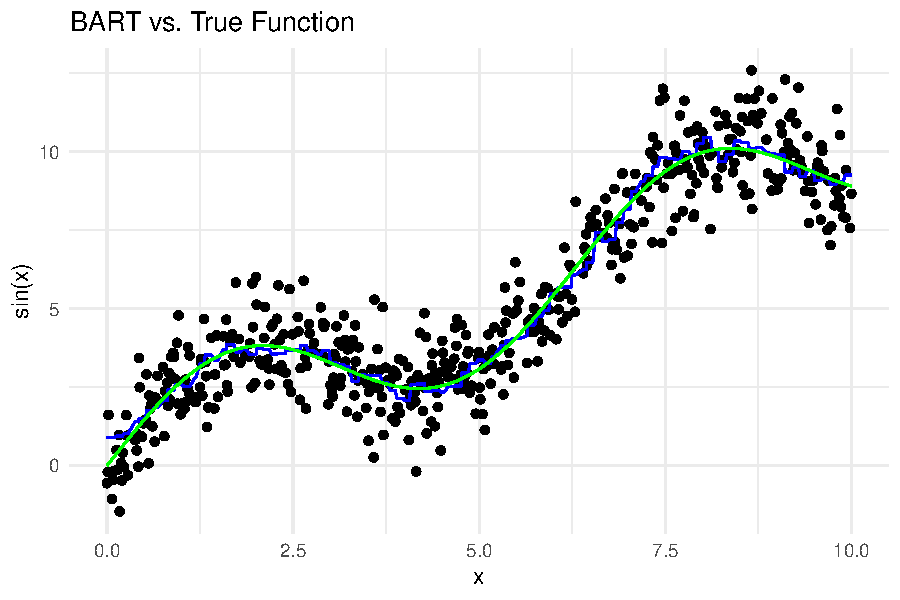
\includegraphics[width=0.7\textwidth]{../outputs/sin_plot.pdf}
  \caption{Plot of the estimates (blue) against observations (black) and generating function(green)}
  \label{plot_sin1}
\end{figure}

To check convergence of the posterior, we plot in figure \ref{plot_sin2} the posterior draws of $\sigma$, the uniquely identified parameter. We observe that the MCMC draw converges quickly to the true parameter, although they oscillate with some autocorrelation due to the posterior sampling procedure.

\begin{figure}
  \centering
  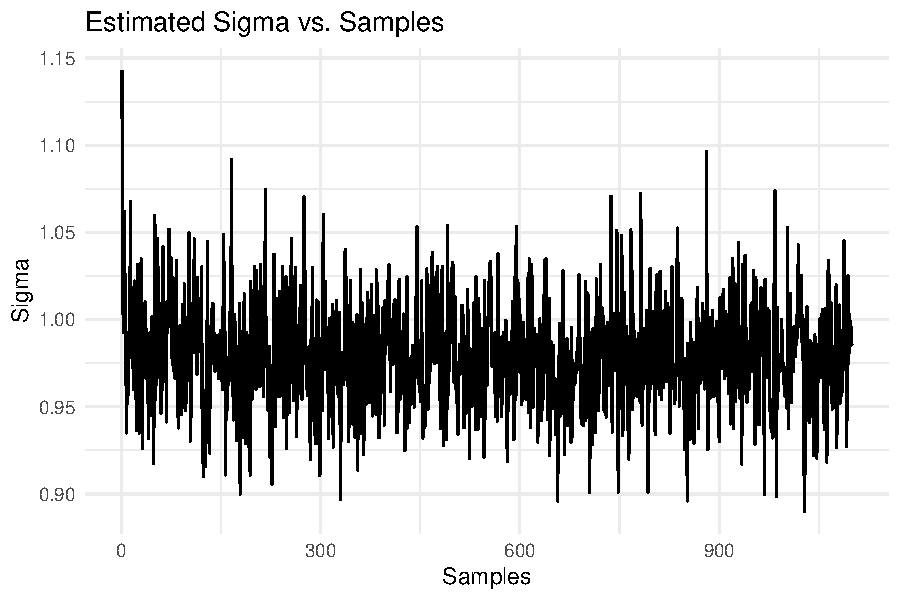
\includegraphics[width=0.7\textwidth]{../outputs/sigma_plot.pdf}
  \caption{Value of $\sigma$ over MCMC iterations}
  \label{plot_sin2}
\end{figure}


To check robustness of BART to different prior specifications, we consider different values for the prior mean of $\sigma$,  that are 100, 0.001 and 1 (the true one). With a large $\sigma$, we observe in plot \ref{plot_sin3} underfitting of the data. With a small $\sigma$, holding all the other parameter constant, the regularization prior is still strong enough to avoid the overfitting.

\begin{figure}
  \centering
  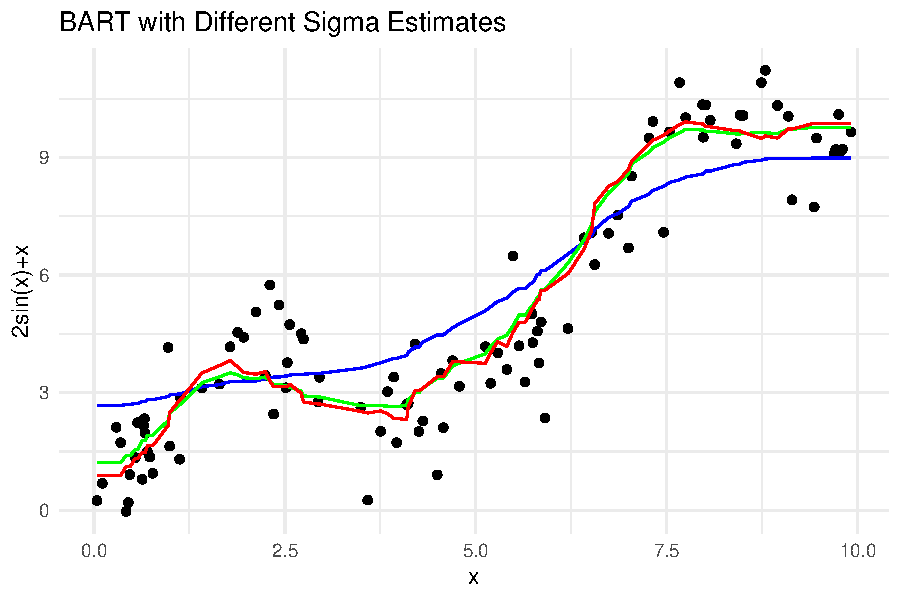
\includegraphics[width=0.7\textwidth]{../outputs/sin_plot_diff_sigma.pdf}
  \caption{DIfferent prior mean of $\sigma$}
  \label{plot_sin3}
\end{figure}


\subsection{Predicting the age of an Abalone}

Abalone are marine snails found in various regions around the world. Determining their age is a labor-intensive process, as it requires cutting through the shell, staining it, and then counting the growth rings under a microscope. However, predicting the age of an abalone can also be done by examining other physical characteristics of the individual, which are much easier to assess. This is precisely the motivation behind our application.

We use data abalone characteristics data coming from the UC Irvine Machine Learning Repository \parencite{warwicknashAbalone1994a}, that is described in table \ref{table1}. No data manipulation is necessary, aside from creating a new variable, \( \text{Age} = \text{Rings} + 1.5 \), and removing the column identifying the number of rings.

\begin{table}[]
  \centering
  \begin{tabular}{llllll}

  \toprule
  Variable Name & Role & Type & Description & Units \\
  \midrule
  Sex                  & Feature       & Categorical   & M, F, and I (infant) & -    \\
  Length               & Feature       & Continuous    & Longest shell measurement & mm\\
  Diameter             & Feature       & Continuous    & Perpendicular to length & mm  \\
  Height               & Feature       & Continuous    & With meat in shell      & mm  \\
  Whole\_weight         & Feature       & Continuous    & Whole abalone           & gram\\
  Shucked\_weight       & Feature       & Continuous    & Weight of meat          & gram\\
  Viscera\_weight       & Feature       & Continuous    & Gut weight (after bleeding) & \\
  Shell\_weight         & Feature       & Continuous    & After being dried       & gram\\
  Rings                & Target        & Integer       & +1.5 gives the age in years & - \\

   \bottomrule
  \end{tabular}
  \caption{Table of Variables}
  \label{table1}
  \end{table}

We run BART from \cite{mccullochBARTBayesianAdditive2024}; Boosting from \cite{ridgewayGbmGeneralizedBoosted2024}; Random Forest and Bagging from \cite{breimanRandomForestBreimanCutlers2024}.Our aim is to compare the predictive performance of those methods. In fact,  we use half of the sample to fit $\hat{y}$, that is the age variable, and half the sample to give us out of bag Mean Squared Errors (MSE) for predicting the same variable. Models are run for various values of T, and for each value, both the mean squared error (MSE) of out-of-sample predictions (shown in plot \ref{plot_mse}) and the computation time (depicted in plot \ref{plot_time}) are recorded.

We observe with a number of trees estimated larger than 500, the BART model is the best performing one, and it reaches also the best performance overall when run with 500 iterations. Although it is the best performer, it is also the model that takes the most to be run, and time of computations scales linearly with the number of trees that are fitted.

\begin{table}[ht]
  \centering
  \begin{tabular}{lcc}
  \toprule
  Model           & MSE & Time (s) \\
  \midrule
  BART            & 4.45    & 66.7  \\
  Random Forest   & 4.53    & 4.74  \\
  Boosting        & 4.87    & 0.220 \\
  Bagging         & 4.54    & 12.4  \\
  \bottomrule
  \end{tabular}
  \caption{Model performance with $T=500$}
  \end{table}


\begin{figure}
  \centering
  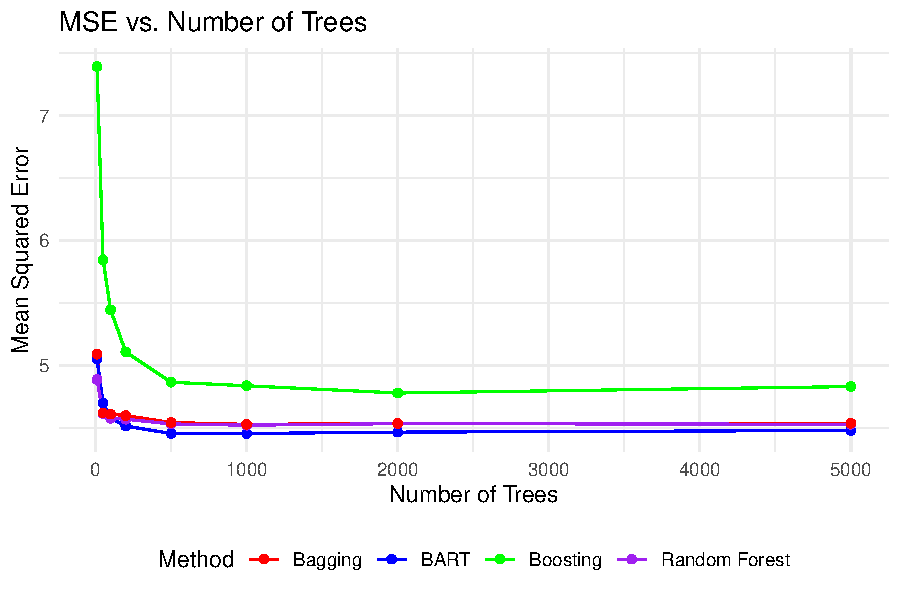
\includegraphics[width=0.7\textwidth]{../outputs/mse_plot.pdf}
  \caption{Mean Squared Error for different values of T}
  \label{plot_mse}
\end{figure}

\begin{figure}
  \centering
  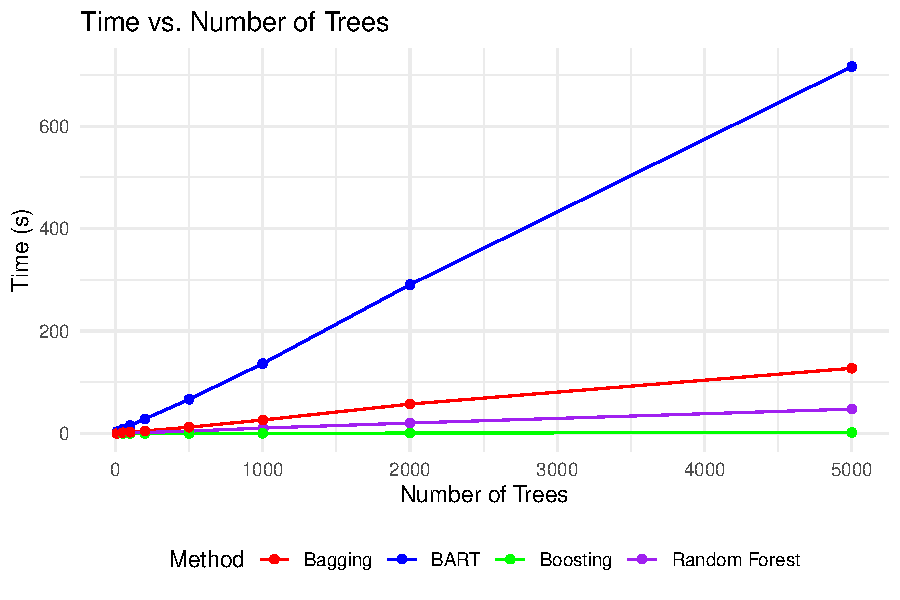
\includegraphics[width=0.7\textwidth]{../outputs/time_plot.pdf}
  \caption{Time of computations for different values of T}
  \label{plot_time}
\end{figure}

\printbibliography

\end{document}